\documentclass[a4paper,twocolumn]{article}
\setlength{\columnsep}{2em}
%\documentclass[paper=a4, fontsize=16pt]{article} % A4 paper and 11pt font size
\usepackage[T1]{fontenc} % Use 8-bit encoding that has 256 glyphs
\usepackage[a4paper, total={7in, 10in}]{geometry}
\usepackage[english, italian]{babel} % English language/hyphenation
\usepackage{amsmath,amsfonts,amsthm} % Math packages
\usepackage[T1]{fontenc}
\usepackage[utf8]{inputenc}
\usepackage{lipsum} % Used for inserting dummy 'Lorem ipsum' text into the template
\usepackage{sectsty} % Allows customizing section commands
\usepackage{graphicx}
\usepackage{epstopdf}
\usepackage{mathtools}
\usepackage{adjustbox}
\usepackage{float}
\usepackage{multicol}
%\setcounter{secnumdepth}{0} %this is to control paragraphs enumeration
\usepackage[italian]{babel}
\usepackage{booktabs}
\usepackage{fancyhdr} % Custom headers and footers
%\usepackage{savetrees}
\usepackage[caption = false]{subfig}
\usepackage{graphicx}
\usepackage{hyperref}

\pagestyle{fancyplain} % Makes all pages in the document conform to the custom headers and footers
\fancyhead{} % No page header - if you want one, create it in the same way as the footers below
\fancyfoot[L]{\small\textsc{Analisi dell'emissione di raggi $\gamma$ dalla pulsar PSR J2021+3651 a.a. 20/21}} % Left footer
\fancyfoot[C]{} % Center footer
\fancyfoot[R]{\thepage} % Page numbering for right footer
\renewcommand{\headrulewidth}{0pt} % Header underlines
\renewcommand{\footrulewidth}{0.3pt} % Foot underlines
\setlength{\headheight}{13.6pt} % Customize the height of the header
\DeclarePairedDelimiter\abs{\lvert}{\rvert}
\DeclarePairedDelimiter\norm{\lVert}{\rVert}

\usepackage{titlesec}
\titleformat{\section}
  {\centering\Large\scshape}{\thesection}{0.5em}{}
\titleformat{\subsection}
  {\centering\normalfont\itshape}{\thesubsection}{0.5em}{}

\usepackage{blindtext}

%----------------------------------------------------------------------------------------
%	SEZIONE TITOLO
%----------------------------------------------------------------------------------------


\begin{document}
	\title{	
	\normalfont \normalsize 
	\textsc{Multimessenger Physics Laboratory  •  a.a. 2020/2021} \\ 
	  [10pt]
	\hrule height 0.4pt
	\bigskip
	%\begin{adobe utopia}
    	\Huge \textbf{Analisi dell'emissione di raggi $\gamma$ dalla pulsar PSR J2021+3651} \\ %Nome dell'esperienza
         [9pt]
    %\end{adobe utopia}	
}
\date{\large{Maggio 2021}}
\author{Sara Ardito}

%----------------------------------------------------------------------------------------
%	TITOLO
%----------------------------------------------------------------------------------------

\maketitle

%----------------------------------------------------------------------------------------
%	INTRODUZIONE
%----------------------------------------------------------------------------------------
\begin{large}

\section{Introduzione}
In questa esperienza si vuole studiare l'emissione periodica di raggi gamma proveniente dalla pulsar PSR J2021+3651, nota come Dragonfly, situata nella nostra Galassia. A tale scopo si esegue l'analisi dei dati raccolti dal \textit{Large Area Telescope} (LAT) a bordo del \textit{Fermi Gamma-ray Telescope} (GLAST).


\subsection{Large Area Telescope}
Il LAT è, con il rivelatore di lampi gamma (GBM), uno degli strumenti che compone il telescopio spaziale \textit{Fermi}. Esso è sensibile alla radiazione gamma nella banda di energia compresa tra 20 MeV e più di 300 GeV e per tale motivo è fondamentale per lo studio dell'emissione gamma da parte delle pulsar. Ha un campo di vista di circa 2.4 sr che corrisponde circa al 20$\%$ del cielo. La risoluzione angolare dipende dall'energia del raggio gamma, dal suo angolo di incidenza e dal punto in cui interagisce nel rivelatore. La PSF per i raggi gamma 'on-axis' ha un raggio di contenimento al 68 $\%$ di circa 3$^{\circ}$ a 100 MeV e 0.04$^{\circ}$ a 100 GeV. L'area effettiva al centro del campo visivo  è di circa 7000 cm$^2$ ad 1 GeV e decresce ad energie minori e maggiori. Infine la sua risoluzione temporale è di 1 $\mu$s.

\subsection{PSR J2921+3651}
La pulsar PSR J2021+3651, scoperta da Robert et al. (2002), presenta caratteristiche simili ad altre pulsar note come la Vela.\\
Si tratta di una pulsar giovane ed energetica, con età caratteristica di 17 kyr, un periodo di 103.7 ms e una luminosità pari a 3.38$\times$10$^{36}$ erg s$^{-1}$ (Abdo et al. 2009).
Alcune stime suggeriscono una distanza D = 12 kpc, mentre la sua posizione nel cielo è nota e secondo quanto riportato nell' \textit{ATNF Pulsar Catalogue} è RAJ = 20$^h$21$^m$05.46$^s$, DECJ = +36$^\circ$51'04.8".\\
Successive osservazioni eseguite con il \textit{Chandra X-ray Observatory} hanno rivelato la presenza di pulsazioni nei raggi X e la formazione di una nebulosa (Pulsar Wind Nebula), la 'Dragonfly Nebula'.

%----------------------------------------------------------------------------------------
%	RACCOLTA DATI
%----------------------------------------------------------------------------------------

\section{Raccolta dati}
Prima di procedere all'analisi della pulsar in esame ho scaricato i dati raccolti dal LAT attraverso il sito web del \textit{Fermi Science Support Center}.\\
Nel portale del Fssc ho selezionato la voce 'LAT Data Server' ed ho inserito le coordinate della pulsar nel formato RA,DEC (20$^h$21$^m$05.46$^s$, +36$^\circ$51'04.8"), ho selezionato un intervallo di energie di 100 MeV - 500 GeV ed un raggio di selezione di 4$^{\circ}$ (questo valore è di poco superiore alla PSF a 100 MeV, che è circa 3$^{\circ}$).\\
Ai fini dell'analisi ho selezionato una finestra di osservazione T = 54730 - 54820 MJD.\\
Terminata la procedura di download ho a disposizione i file relativi agli eventi e allo spacecraft in formato fits.
A questo punto ho eseguito un'ulteriore selezione dei dati usando i Fermi tools: con \textit{gtselect} ho selezionato la classe dei fotoni e il tipo (evclass=128, evtype=3), ho scelto un raggio di 3$^{\circ}$, un'energia minima di 100 MeV ed il massimo valore dello zenith angle a 90$^{\circ}$ in modo da ridurre i fotoni dell'albedo terrestre. Inoltre ho selezionato i fotoni con tempi di arrivo compresi tra 1000 s dopo l'inizio del file FT2 e 1000 s prima della fine del file FT2 (start time = 243649001 s, end time = 251423001).\\
Successivamente ho usato il tool \textit{gtgmktime} in modo da rimuovere i fotoni esterni ai Good Time Intervals (GTIs).

%----------------------------------------------------------------------------------------
%	COUNT MAP
%----------------------------------------------------------------------------------------


\section{Count Map}
Con i file filtrati è possibile realizzare una mappa dei fotoni per diversi range di energia.\\
Se si considerano fotoni con energia E< 300 MeV si rischia di confondere l'emissione della pulsar con la radiazione proveniente dal background e dalle sorgenti vicine.\\
Quindi ho selezionato i fotoni con energia E > 300 MeV e ho realizzato un istogramma bidimensionale ponendo sulle x la coordinata RA e sulle y la coordinata DEC dei fotoni. Per realizzare la mappa in Figura \ref{cmap300} ho utilizzato 80 bins in entrambe le direzioni.


\begin{figure}[h]
    \makebox[\linewidth][c]{\includegraphics[scale=0.6]{../results/cmap300.png}}
    \caption{\small Mappa dei fotoni per energie E > 300 MeV. La croce in rosso indica la posizione della pulsar PSR J2021+3651 secondo l'\textit{ATNF pulsar catalogue}.}
    \label{cmap300}
\end{figure}


\noindent
La pulsar PSR J2021+3651 è centrata nella figura precedente, infatti il centro della figura, cioè la semidifferenza del valore massimo e minimo delle coordinate, è (RA, DEC) = (305.278, 36.851) ed è compatibile con le coordinate della sorgente riportate nell'\textit{ATNF pulsar catalogue} (RA, DEC)$_{catalog}$ = (305.272, 36.851) convertite in unità 'deg'.\\
Dal grafico emerge che l'emissione di raggi gamma è concentrata nella zona centrale, cioè in corrispondenza della sorgente.
Un'ulteriore prova è data dalla Figura \ref{c_dist} in cui riporto la distribuzione delle coordinate dei fotoni. Le due curve seguono lo stesso andamento: presentano un picco centrale e decrescono lungo le code. In prima approssimazione possiamo considerare le due distribuzioni simmetriche e nel caso della coordinata RA la media e la deviazione standard sono (305.27 $\pm$ 2.18) deg, mentre per la coordinata DEC si ha (36.85 $\pm$ 1.74). Tali valori sono compatibili con le coordinate della pulsar.

\begin{figure}[h]
    \makebox[\linewidth][c]{\includegraphics[scale=0.55]{../results/coord_distribution.png}}
    \caption{\small Distribuzione della coordinata RA (in alto) e della coordinata DEC (in basso) dei fotoni con energia E > 300 MeV. La finestra in verde è centrata nel valore medio e ha larghezza pari al doppio della deviazione standard. Entrambi gli istogrammi sono stati realizzati con 100 bins.}
    \label{c_dist}
\end{figure} 

\noindent 
È anche possibile studiare la distribuzione dei fotoni in funzione della distanza dal centro dell'immagine, il risultato è riportato in Figura \ref{d300}. 

\begin{figure}[h]
    \makebox[\linewidth][c]{\includegraphics[scale=0.55]{../results/d300_distribution.png}} 
    \caption{\small Distribuzione della distanza dei fotoni dal centro dell'immagine. L'istogramma è stato realizzato con 100 bins.}
    \label{d300}
\end{figure}

\noindent
Si vede che i fotoni sono distribuiti in un intervallo di poco superiore a 3$^{\circ}$, con un picco in corrispondenza di 3$^{\circ}$ e una rapida decrescita per valori superiori. Questo valore ricorda molto la PSF per i raggi gamma 'on-axis' che ha un raggio di contenimento al 68$\%$ di circa 3$^{\circ}$ a 100 MeV e decresce all'aumentare dell'energia.\\
In seguito ho realizzato una mappa dei fotoni analoga alla precedente ma selezionando fotoni con energia E > 1 GeV (Figura \ref{cmap1G}).

\begin{figure}[h]
    \makebox[\linewidth][c]{\includegraphics[scale=0.6]{../results/cmap1G.png}} 
    \caption{\small Mappa dei fotoni per energie E > 1 GeV. La croce in rosso indica la posizione della pulsar PSR J2021+3651 secondo l'\textit{ATNF pulsar catalogue}.}
    \label{cmap1G}
\end{figure}

\noindent
Si nota una diminuzione del numero di fotoni nella zona che circonda la sorgente, ciò è evidente negli gli istogrammi in Figura \ref{c_dist1}, che rappresentano come sono distribuiti i fotoni per le coordinate RA e DEC.
Questi presentano delle code meno dense e con una decrescita più rapida rispetto a quanto visto precedentemente per fotoni con E > 300 MeV.
In effetti lo spettro della pulsar PSR J2021+3651 presenta un cut-off esponenziale per energie superiori ad 1 GeV (Abdo et al. 2009).


\begin{figure}[h]
    \makebox[\linewidth][c]{\includegraphics[scale=0.56]{../results/coord_distribution1G.png}} 
    \caption{\small Distribuzione della coordinata RA (in alto) e della coordinata DEC (in basso) dei fotoni con energia E > 1 GeV. La finestra in verde è centrata nel valore medio e ha larghezza pari al doppio della deviazione standard. Entrambi gli istogrammi sono stati realizzati con 100 bins.}
    \label{c_dist1}
\end{figure}
 
\noindent
Infine in Figura \ref{d1G} ho riportato la distribuzione dei fotoni in funzione della distanza dal centro dell'immagine. Notiamo che il numero dei conteggi è diminuito rispetto al caso precedente, segno del fatto che vi sono meno fotoni di alta energia, ed è visibile un primo picco a $\sim$0.3$^{\circ}$, che infatti corrisponde alla zona in cui vi è una maggiore emissione di fotoni.

\begin{figure}[h]
    \makebox[\linewidth][c]{\includegraphics[scale=0.55]{../results/d1G_distribution.png}}
    \caption{\small Distribuzione della distanza dei fotoni dal centro dell'immagine per E > 1 GeV. L'istogramma è stato realizzato con 100 bins.}
    \label{d1G}
\end{figure}


%----------------------------------------------------------------------------------------
%	RICERCA DI PERIODICITÀ
%----------------------------------------------------------------------------------------

\section{Ricerca di periodicità}
Per poter procedere con l'analisi è necessario applicare le correzioni baricentriche al file FT1 usato nella sezione precedente. Infatti i tempi di arrivo dei fotoni , espressi in Terrestrial Time (TT), sono affetti da errori dovuti al moto del GLAST nel Sistema Solare e da effetti relativistici. Pertanto ho utilizzato il tool \textit{gtbary}, che converte i tempi di arrivo in tempi di arrivo nel baricentro del Sistema Solare (Barycentric Dynamical Time TDB).  \\
A questo punto si può fare la ricerca di periodicità e trovare la frequenza e la sua derivata prima, necessarie per calcolare le fasi dei fotoni (eq. \ref{fasi}) e realizzare il fasogramma. Per fare ciò ho effettuato il test di periodicità Z$^2_{n}$ con un numero di armoniche n = 8:
\begin{equation}
Z^2_n = \frac{2}{N} \sum\limits_{k=1}^n \left(\sum\limits_{i=1}^N cos(k\phi_i)\right)^2 + \left(\sum\limits_{i=1}^N sin(k\phi_i)\right)^2
\end{equation}

\begin{equation}
\phi_i = f_0 (t-T_0) + \frac{f_1}{2} (t-T_0)^2  \quad i = 1,N
\label{fasi}
\end{equation}

\noindent
dove N è il numero di fotoni ed ho usato come epoca T$_0$ il tempo centrale dell'intervallo di osservazione, T$_0$ = 247536001 s, e come valori centrali f$_0^{start}$ = 9.63935 Hz ed f$_1^{start}$ = -8.8892 $\times$ 10$^{-12}$ Hz/s. Quindi ho effettuato una scansione bidimensionale su f$_0$ ed f$_1$ considerando una spaziatura df$_0$ = 0.15/T Hz e df$_1$ = 0.3/T$^2$ Hz/s con T = 7776000 s uguale alla durata dell'intervallo di osservazione. Inoltre ho eseguito 1000 tentativi su f$_0$ e 50 su f$_1$.
Al termine della scansione ho ottenuto i parametri rotazionali ottimali riportati in Tabella \ref{ztest}.

\begin{table}[H]
\caption{\small Effemeridi della pulsar PSR J2021+3651.}
\begin{tabular}{lc}
\hline
\hline
Nome & J2021+3651\\
Ascensione retta (J2000) & 20$^h$21$^m$05.46$^s$\\
Declinazione (J2000) &  +36$^\circ$51'04.8"\\
Frequenza f$_0$ (Hz) & 9.6393449\\
Derivata della frequenza f$_1$ (Hz/s) & -8.8891999 $\times$ 10$^{-12}$\\
Epoca di osservazione (MJD) & 54730-54820\\
Massimo Z$^2_n$ test & 1253.8119\\
\hline
\end{tabular}
\label{ztest}
\end{table}

\noindent
In Figura \ref{scan} riporto lo scan di periodicità ponendo sugli assi il numero dei passi della scansione. Si vede che il massimo dello Z$^2_n$ test si ha in corrispondenza dello step 237 per f$_0$ e dello step 25 per f$_1$.

\begin{figure}[h]
    \makebox[\linewidth][c]{\includegraphics[scale=0.6]{../results/scan.png}} 
    \caption{\small Scan per la ricerca di periodicità.}
    \label{scan}
\end{figure}

\noindent
Per assodare la correttezza dei valori f$_0$ ed f$_1$ ho realizzato uno scatter plot (Figura \ref{scatter}) ponendo sull'asse x la fase dei fotoni, valutata in corrispondenza dei parametri rotazionali ottimali, e sulle y il tempo di arrivo espresso in MET. Per chiarezza ho riportato sull'asse x due periodi.\\
Prendendo in esame un solo periodo notiamo la formazione di due linee verticali in corrispondenza di $\phi \sim$ 0.13 e $\phi \sim$ 0.6. Quindi ne deduciamo che in corrispondenza di questi valori si osserva un maggior numero di fotoni, inoltre le linee verticali appaiono dritte lungo tutto l'intervallo di osservazione, ciò significa che non si sono verificati glitch o fenomeni che hanno come conseguenza una variazione della fase degli impulsi gamma emessi dalla pulsar.


\begin{figure}[h]
    \makebox[\linewidth][c]{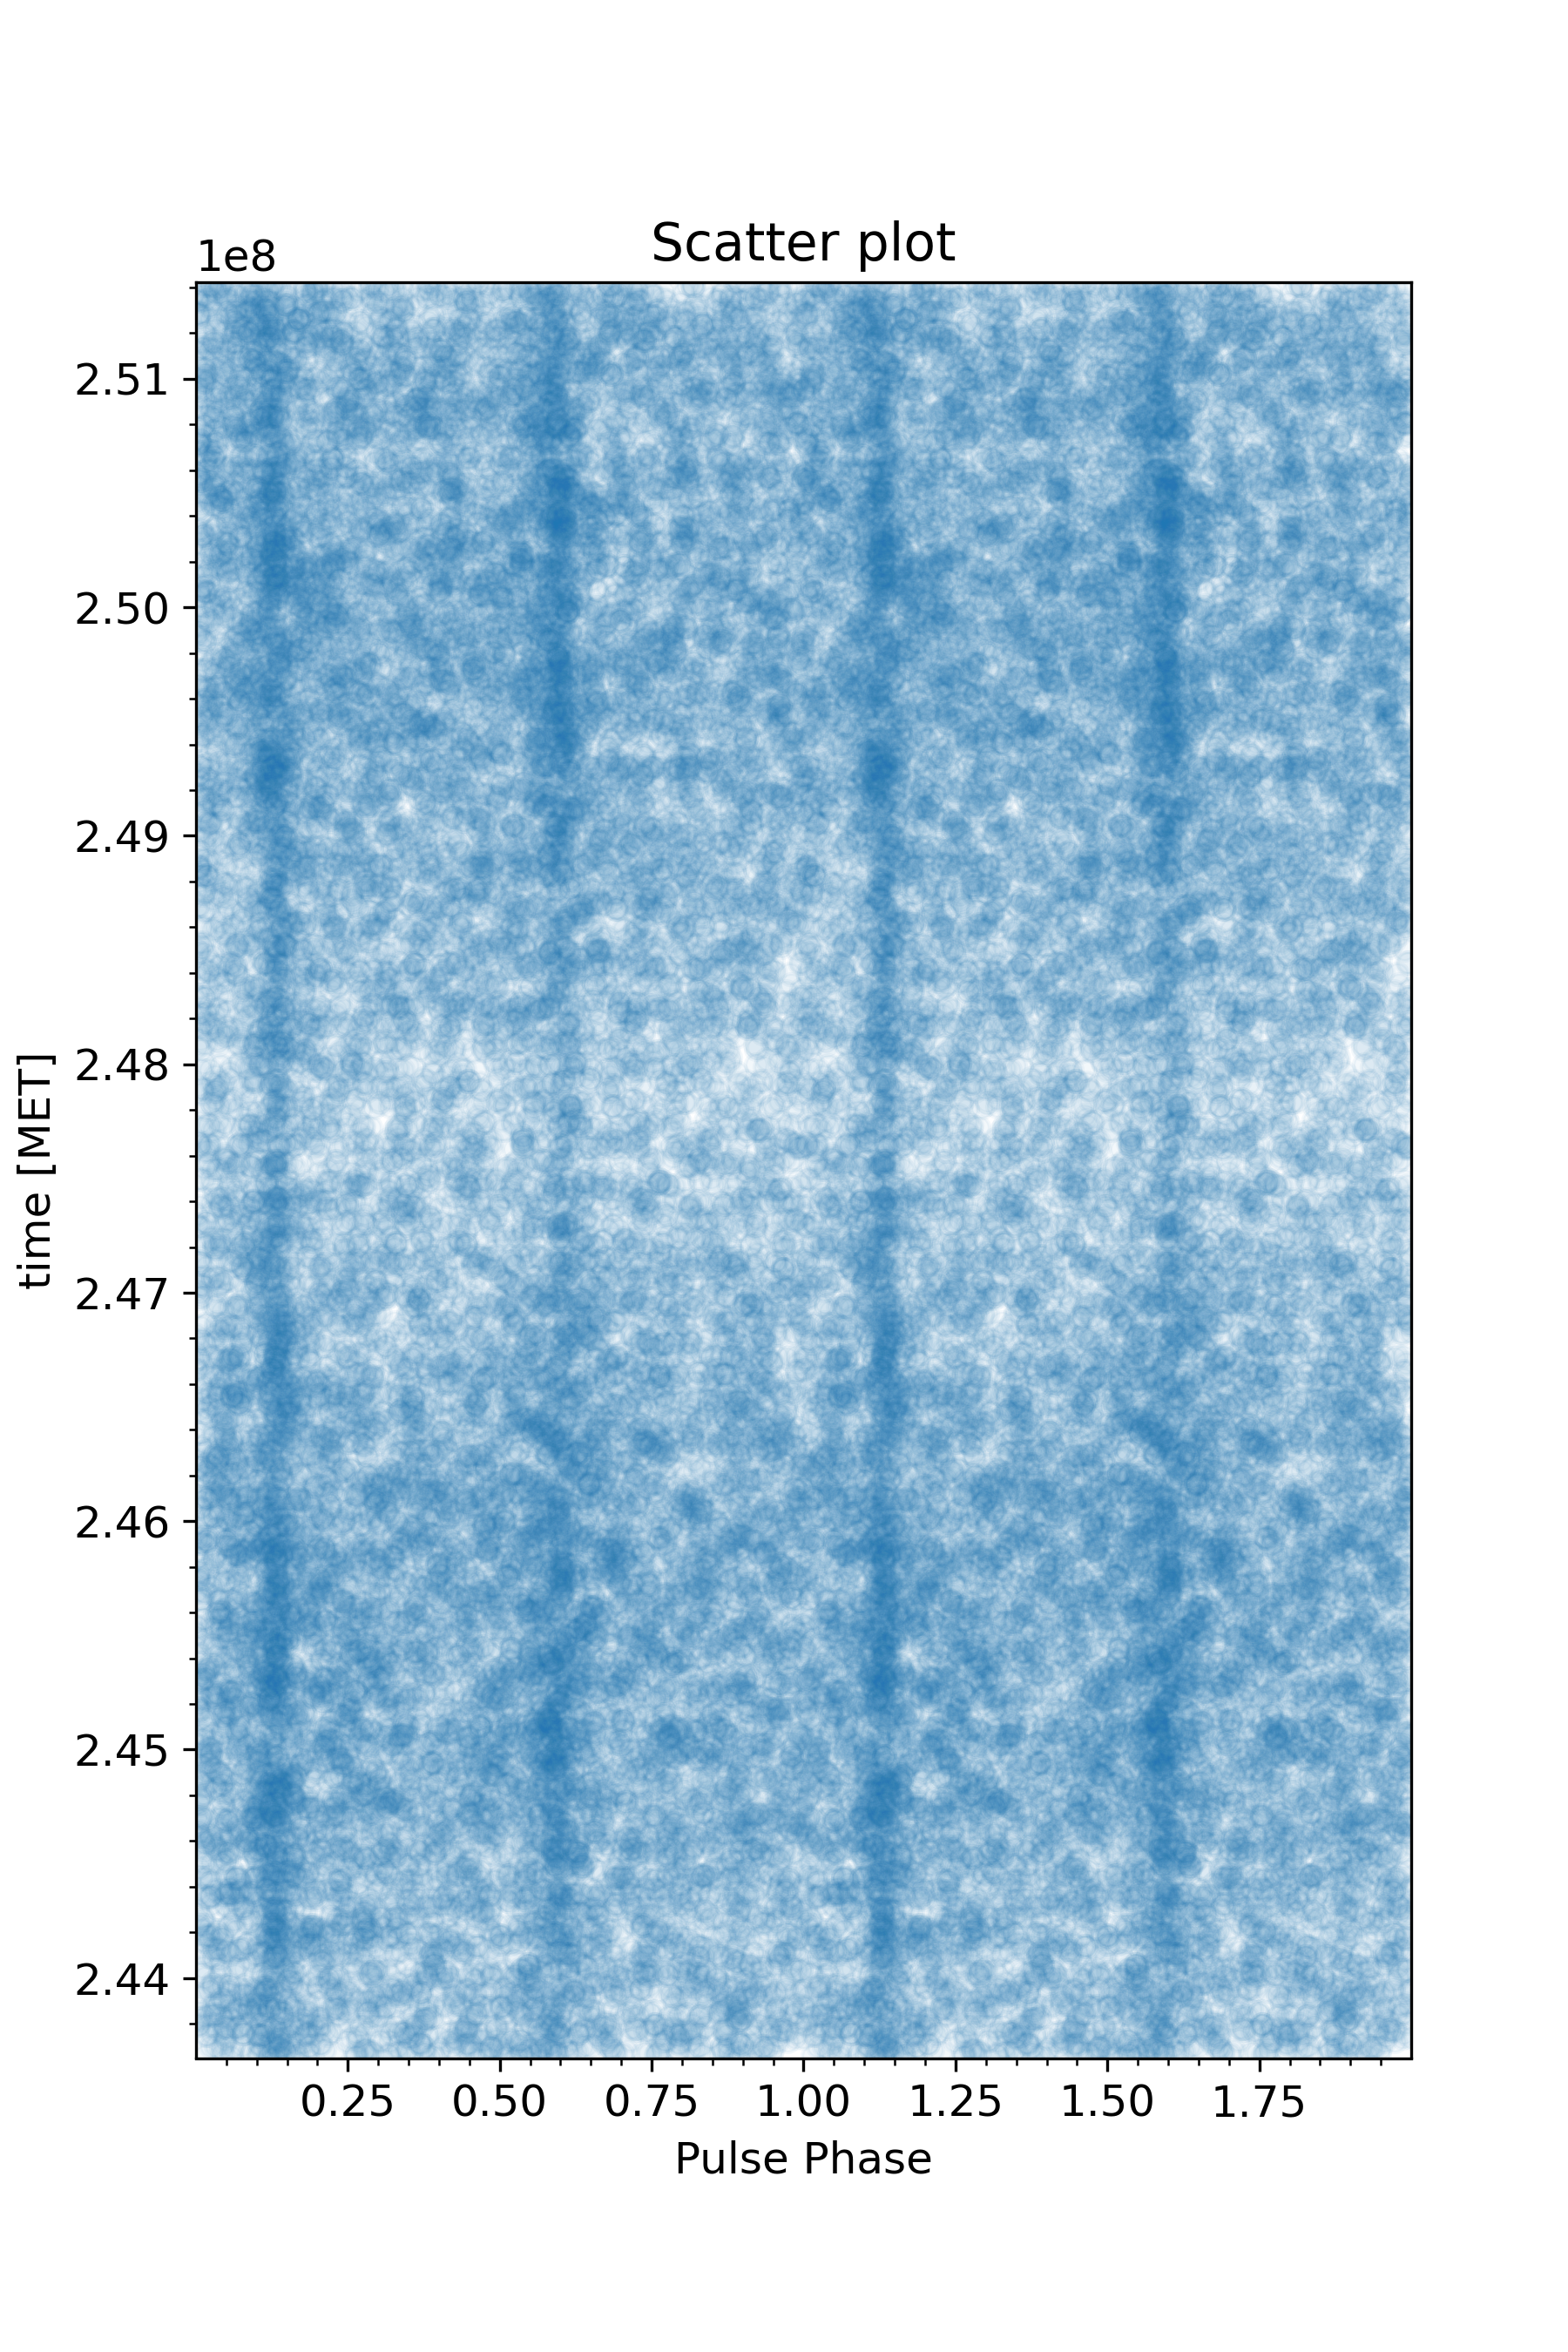
\includegraphics[scale=0.6]{../results/scatterplot.png}} 
    \caption{\small Scatter plot dei fotoni rivelati durante tutto il periodo osservativo. Sull'asse delle x sono riportati due periodi di rotazione.}
    \label{scatter}
\end{figure}

%----------------------------------------------------------------------------------------
%	FASOGRAMMI
%----------------------------------------------------------------------------------------
\section{Istogramma delle fasi}
Usando i parametri rotazionali ottimali, che mi hanno restituito il valore più grande dello Z$^2_n$, ho calcolato le fasi (eq. \ref{fasi}) e ne ho preso la parte frazionaria.\\
Ho successivamente realizzato un fasogramma complessivo per tutti i fotoni con energia E > 0.1 GeV, riportando sull'asse delle x due cicli di rotazione.\\
Il risultato è mostrato in Figura \ref{phas1}.

\begin{figure}[h]
%\centering
    \makebox[\linewidth][c]{\includegraphics[scale=0.6]{../results/phasogram1.png}} 
    \caption{\small Fasogramma per raggi gamma con E > 100 MeV. Ogni bin ha una larghezza di 0.01 in fase e sulle x sono riportati due cicli di rotazione. La linea tratteggiata mostra il valore medio dei conteggi nel background.}
    \label{phas1}
\end{figure}

\noindent
Si notano due picchi che in prima approssimazione coprono un range di fasi rispettivamente di 0.08 < $\phi_1$ < 0.21 e 0.52 < $\phi_2$ < 0.68. Questi range corrispondono alle finestre che evidenziano la presenza del picco in Figura \ref{fasi}.\\
Ho usato queste finestre per mascherare i picchi e calcolare media e deviazione standard dei conteggi di background $bckg$ = 232 $\pm$ 31. Quindi ho deciso di attribuire a ciascuna fase un'incertezza $d\phi$ = 0.01, uguale alla larghezza del bin, e a ciascun conteggio $dcount$ = 1$\sigma$ = 31.\\
Entrambi i picchi possono essere fittati con una Lorentziana (Figura \ref{fit}):

\begin{equation}
y = \frac{A}{\pi} \frac{(\Gamma /2)^2}{(\Gamma /2)^2 + (x - x_0)^2} + cost
\end{equation}
dove $\Gamma$ è la larghezza a metà altezza (FWHM) e $x_0$ il centro del picco.\\


\begin{figure}[h]
%\centering
    \makebox[\linewidth][c]{\includegraphics[scale=0.55]{../results/fitLor.png}} 
    \caption{\small Fit dei due picchi usando una Lorentziana. Le barre di errore sui conteggi corrispondono ad 1 $\sigma$.}
    \label{fit}
\end{figure}

\noindent
Ho deciso di realizzare il fit per i due picchi separatamente, escludendo cioè la fase di 'off-pulse' e considerando solo le finestre dei due picchi.\\
I risultati di maggiore interesse dei fit sono riportati in Tabella \ref{fitT}:

\begin{table}[H]
\centering

\begin{tabular}{lccc}
\hline
\hline
 & $\phi_0$ & FHWM & cost \\
\hline
Peak 1 & 0.124 $\pm$ 0.001 &  0.031 $\pm$ 0.003 & 230 $\pm$ 6 \\
Peak 2 & 0.589 $\pm$ 0.001 &  0.042 $\pm$ 0.005 & 231 $\pm$ 9 \\
\hline
\end{tabular}
\caption{\small Risultati dei fit.}
\label{fitT}
\end{table}

\noindent
Usando i valori centrali dei picchi ho stimato una separazione di fase $\delta \phi$ = $\phi_0^{peak2}$ - $\phi_0^{peak1}$ = 0.46 $\pm$ 0.02. Per stimare l'errore ho deciso di attribuire alla fase di ciascun picco un'incertezza pari alla metà della larghezza del picco FHWM, ho poi sommato in quadratura i valori delle due incertezze.\\
L'altezza di ciascun picco, H$_1$ $\sim$ 333 ed H$_2$ $\sim$ 260, è stata calcolata valutando il valore massimo della funzione Lorentziana in corrispondenza dei parametri di fit ottimali e sottraendo a tale valore il valore medio del background. Quindi si ottiene un rapporto $H_1/H_2$ $\sim $1.28.\\
Notiamo che tutti i valori in Tabella \ref{fitT} sono compatibili entro due sigma con i valori ottenuti da Abdo et al. (2009).\\
Infine ho realizzato dei fasogrammi per diversi range di energia e ho riportato il risultato in Figura \ref{Eband}. Notiamo che la posizione dei due picchi rimane costante all'aumentare dell'energia, mentre il valore medio dei conteggi di background tende a diminuire, come  avevamo già constatato con la count map.\\
Per quanto riguarda i picchi vediamo che il numero dei conteggi diminuisce all'aumentare dell'energia, tuttavia il primo picco continua ad essere più intenso del secondo in ogni range di energia. Si nota inoltre che il secondo picco diventa meno evidente ad energie più basse mentre il primo picco persiste.  

\begin{figure*}[h]
\centering
    \includegraphics[scale=0.5]{../results/E_band.png} 
    \caption{\small Fasogrammi per diverse bande di energia. Ogni bin ha una larghezza di 0.01 in fase e sulle x sono riportati due cicli di rotazione. La linea tratteggiata mostra il valore medio dei conteggi nel background, invece le due linee verticali corrispondono alla posizione centrale dei picchi tabulata in Tabella \ref{fitT}.}
    \label{Eband}
\end{figure*}

%----------------------------------------------------------------------------------------
%	CARATTERIZZAZIONE DELLA PULSAR
%----------------------------------------------------------------------------------------
\section{Caratterizzazione della pulsar}
Una volta noti i parametri rotazionali ottimali è possibile determinare le quantità caratteristiche della pulsar. In Tabella \ref{catalog} riporto le caratteristiche della pulsar PSR J2021+3651 tabulate nell'\textit{ATNF pulsar catalogue}.

\begin{table}[H]
\caption{\small Caratteristiche della pulsar PSR J2021+3651.}
\begin{tabular}{lc}
\hline
\hline
Nome & J2021+3651\\
Periodo P$_0$ (s) & 0.1037\\
Derivata del Periodo P$_1$  & 9.57 $\times$ 10$^{-12}$ \\
Frequenza f$_0$ (Hz) & 9.639348581\\
Derivata della frequenza f$_1$ (Hz/s) & -8.89419 $\times$ 10$^{-12}$\\
Età di dipolo (yr) & 1.72 $\times$ 10$^{4}$\\
Bsurf (G) & 3.19 $\times$ 10$^{12}$\\
Edot (erg/s) & 3.4 $\times$ 10$^{36}$\\ 
\hline
\end{tabular}
\label{catalog}
\end{table}

\noindent
Usando il modello di emissione di dipolo per le pulsar è possibile dare una stima delle quantità sopra citate. Ricordando che P = 1/f$_0$ e $\dot{P}$ = - f$_1$/f$_0^2$ si ha P $\sim$ 0.103741 s e $\dot{P} \sim$ 9.566821 $\times$ 10$^{-14}$ s. Quindi l'età caratteristica è

\begin{equation}
\tau = \frac{P}{2 \dot{P}} = 17.2 \mbox{kyr},
\end{equation}

il campo magnetico B è 

\begin{equation}
B_p = 3.2 \times 10^{19} \left(P \dot{P} \right)^{1/2} = 3.187 \times 10^{12} \mbox{G}
\end{equation}

infine la luminosità è

\begin{equation}
\frac{dE}{dt} = 4 \pi 2 I \frac{\dot{P}}{P^3} = 3.383 \times 10^{36} \mbox{erg/s}
\end{equation}

\noindent
con I = 10$^{45}$ g/cm$^2$, momento di inerzia tipico di un oggetto compatto.
A questo punto è possibile costruire un diagramma P-$\dot{P}$ di tutte le pulsar radio note. Quindi ho scaricato il catalogo dell'$\textit{ATNF}$ e ho rappresentato tutte le pulsar nel plot in Figura \ref{PPdot}.\\
Nel grafico ho riportato le linee di uguale luminosità, campo magnetico ed età caratteristica. Da un'analisi approssimativa si può dire che la pulsar PSR J2021+3651 è giovane ed appartiene alle poche pulsar con luminosità superiore ad un valore dell'ordine di 10$^{34}$ erg/s.\\
Non ho riportato nel diagramma la 'death-line' poichè in letteratura l'equazione che definisce tale limite non è ben determinata, infatti dipende dal modello di emissione scelto per la pulsar e dall'equazione di stato.


\begin{figure}[H]
    \makebox[\linewidth][c]{\includegraphics[scale=0.55]{../results/PPdot.png}} 
    \caption{\small Diagramma P-Pdot delle pulsar catalogate nell'$\textit{ATNF catalogue}$. In rosso è indicata la pulsar PSR J2021+3651 oggetto di studio.}
    \label{PPdot}
\end{figure}


%----------------------------------------------------------------------------------------
%	CONCLUSIONI
%----------------------------------------------------------------------------------------
\section{Conclusioni}
L'analisi eseguita sulla pulsar PSR J2021+3651 ha assodato la presenza di due picchi nella curva di luce. Questa caratteristica sembra essere una proprietà comune ad alcune pulsar e si suppone essere la conseguenza dell'emissione di radiazione dalle calotte polari della pulsar, il cui asse magnetico è inclinato rispetto all'asse di rotazione e questo fa sì che entrambi i coni investano l'osservatore entro ciascun periodo.\\
I fasogrammi da me ottenuti sono analoghi a quelli riportati nell'articolo di Abdo et al. (2009), seguono lo stesso andamento all'aumentare l'energia, tuttavia il numero dei conteggi risulta essere maggiore. Ciò può essere dovuto alla scelta del numero dei bins o alla diversa durata del periodo di osservazione, in particolare nell'analisi da me effettuata ho registrato un maggior numero di conteggi nel background probabilmente a causa di radiazione proveniente da sorgenti vicine.\\
Una difficoltà che ho riscontrato nel corso dell'analisi è stata individuare l'incertezza da associare ai conteggi a causa dell'arbitrarietà del numero dei bins, per cui ho deciso di considerare come errore 1 $\sigma$. Tale scelta ha come conseguenza il fatto che il $\chi^2_{red}$ ottenuto nei due fit sia minore di 1, infatti ho ottenuto $\chi^2_{red}$ = 0.319 per il primo picco e $\chi^2_{red}$ = 0.338 per il secondo picco. Questo sembra essere un caso di overfitting.\\
In conclusione i risultati ottenuti da questa analisi sono compatibili con quanto riportato in letteratura.

\end{large}
\end{document}

